\documentclass{handout}

%\SetInstructor{Capt Steven Beyer}
\SetCourseTitle{ECE210: Introduction to Electrical and Computer Engineering}
\SetHandoutTitle{Robot PCB}

%\ShowAllBlanks

\usepackage[obeyspaces]{url}

\graphicspath{{./figs/}}

%\showsoln \setsolncolor{red}

\begin{document}
	%	\footnotetext{Examples are abstracted from Tutorials Point, "Arduino", 2019, accessed Feb 18, 2019. [Online]. Available: https://www.tutorialspoint.com/arduino/index.htm}
	\maketitle
	
	\section{Objectives.} 
	\begin{enumerate}
		\item Demonstrate the ability to build a robotics system using Electrical and Computer Engineering (ECE) fundamentals such as soldering, assembly, and fabrication.
		\item Troubleshoot ECE applications utilizing modern test equipment.
	\end{enumerate}
	
	\section{Materials.}
	\begin{enumerate}
		\item Printed Circuit Board (PCB)
		\item 1 - $330\ k\Omega$ resistor (R1)
		\item 5 - $10\ k\Omega$ resistors (R2 - R6)
		\item 1 - $13\ k\Omega$ resistor (R7)
		\item 1 - $1\ k\Omega$ resistor (R8)
		\item 3 - $0.1\ \mu F$ ceramic disc capacitors (C1-C3)
		\item 1 - $10\ \mu F$ radial capacitor (C4)
		\item 1 - $33\ \mu F$ radial capacitor (C5)
		\item 2 - 2N3904 transistors (Q1-Q2)
		\item 1 - 2N3906 transistor (Q3)
		\item 1 - L7805 $5\ V$ voltage regulator (U1)
		\item 1 - L78L33 $3.3\ V$ voltage regulator (U2)
		\item 2 - red LEDs
		\item Headers
		\begin{enumerate}
			\item 4 - 1x2 male headers (J1-J4)
			\item 2 - 1x2 female headers (J5 and J6)
			\item 1 - 2x5 female header (Power Connector)
			\item 2 - 8x1 female headers (Motor Driver)
		\end{enumerate}
		\item Motor Driver
		\begin{enumerate}
			\item Motor Driver Board
			\item 2 - 8x1 male headers
		\end{enumerate}
	\end{enumerate}

\newpage
\clearpage
\pagebreak
	
	\section{PCB}
	Your PCB should look like the below figure with all components labeled. This PCB provides power and motor functionality for your robot.
		\begin{figure} [H]
			\centering
			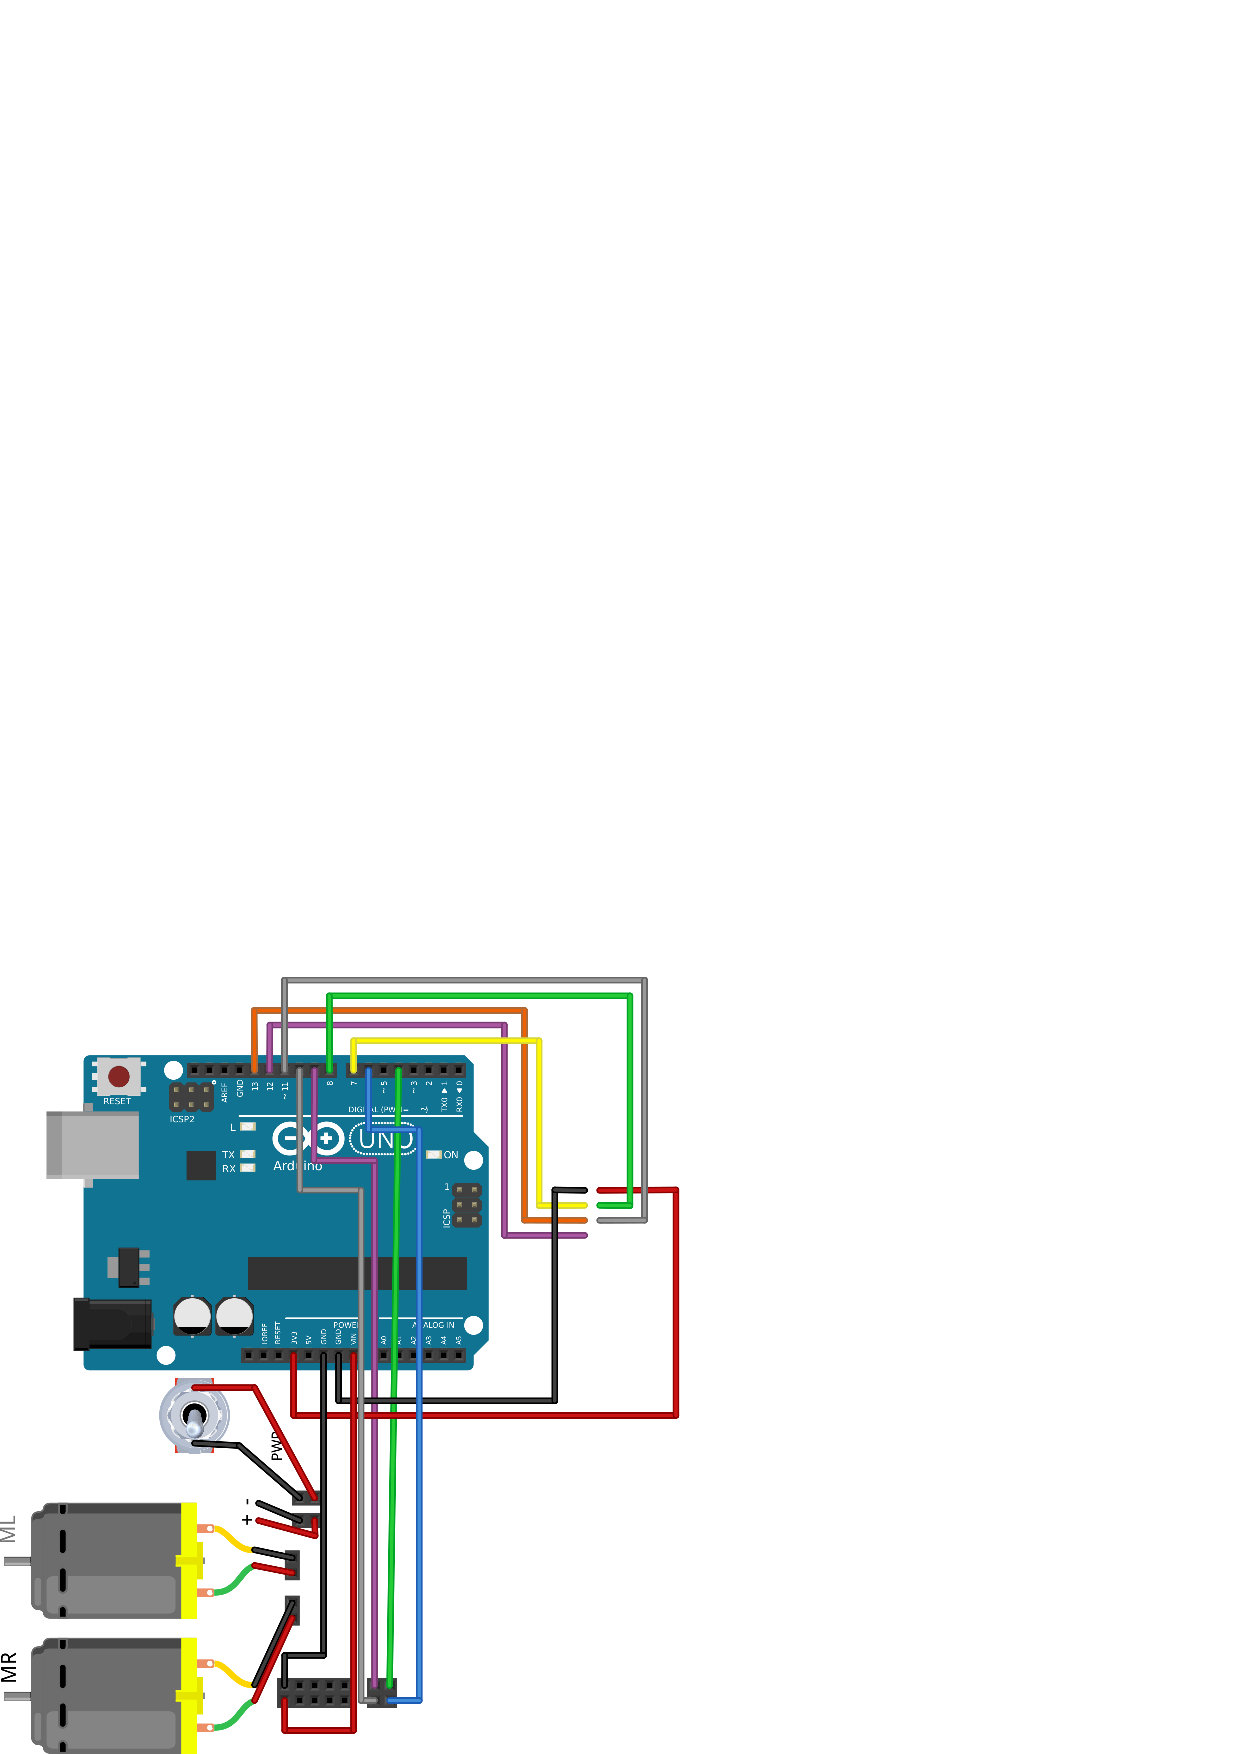
\includegraphics[width=.75\textwidth]{robot.png}
			\caption{Printed Circuit Board}
		\end{figure}
	
	
	\section{Resistors}
	Gather the 8 resistors. Confirm actual resistance using the digital multimeter (DMM). These are non-directional. Solder each onto the board.
	
	\begin{figure} [H]
		\centering
		\includegraphics[width=.5\textwidth]{resistors.jpg}
		\caption{Resistors}
	\end{figure}
	
	\section{Ceramic Disc Capacitors}
	Gather the 3 ceramic disc capacitors. These are non-directional. Solder each onto the board.
	
	\begin{figure} [H]
		\centering
		\includegraphics[width=.5\textwidth]{disccapacitors.jpg}
		\caption{Ceramic Disc Capacitors}
	\end{figure}
	
	\newpage
	\clearpage
	\pagebreak
	
	\section{Radial Capacitors}
	Gather the 2 radial capacitors. These are directional. The negative sign on the capacitor cap should be oriented opposite the positive on the board. Solder each onto the board.
	
	\begin{figure} [H]
	\centering
	\includegraphics[width=.5\textwidth]{radialcapacitors.png}
	\caption{Radial Capacitors}
	\end{figure}

	\section{Transistors}
	Gather the 3 transistors. These are directional. The flat edge of the transistor should correspond with the board. Solder each onto the board.
	
	\begin{figure} [H]
		\centering
		\includegraphics[width=.5\textwidth]{transistors.png}
		\caption{Transistors}
	\end{figure}
	
	\section{5 V Voltage Regulator}
	Gather the $5\ V$ voltage regulator. Use pliers to bend the leads $90^o$ towards the back of the regulator (flat side) at the point that the lead thins. Place the regulator so that the flat side lays flat on the top of the PCB. Solder it onto the board.
	
	\begin{figure} [H]
		\centering
		\includegraphics[width=.5\textwidth]{5vreg.png}
		\caption{$5\ V$ Voltage Regulator}
	\end{figure}

\newpage
\clearpage
\pagebreak

	\section{3.3 V Voltage Regulator}
	Gather the $3.3\ V$ voltage regulator. This is directional. The flat edge of the regulator should correspond with the board. Solder it onto the board.
	
	\begin{figure} [H]
		\centering
		\includegraphics[width=.5\textwidth]{33vreg.png}
		\caption{$3.3\ V$ Voltage Regulator}
	\end{figure}
	
	\section{LEDs}
	Gather the 2 LEDs. Use the DMM to make sure both are operational. These are directional. The flat edge of the LED and the long lead should be oriented toward the negative on the board. Solder them onto the board.
	
	\begin{figure} [H]
		\centering
		\includegraphics[width=.5\textwidth]{leds.png}
		\caption{LEDs}
	\end{figure}
	
	\section{Male Headers}
	Gather the 4 - 1x2 male headers. The smaller end of the header should go through the board. Solder them onto the board.
	
	\begin{figure} [H]
		\centering
		\includegraphics[width=.5\textwidth]{maleheaders.png}
		\caption{Male Headers}
	\end{figure}

\newpage
\clearpage
\pagebreak

	\section{Female Headers}
	Gather the 5 female headers. Solder them onto the board.
	
	\begin{figure} [H]
		\centering
		\includegraphics[width=.5\textwidth]{femaleheaders.png}
		\caption{Female Headers}
	\end{figure}

	\section{PCB with No Motor Driver Board}
	Your board should look like the below figure at this point.
	\begin{figure} [H]
		\centering
		\includegraphics[width=.5\textwidth]{pcb0.png}
		\caption{PCB with No Motor Driver Board}
	\end{figure}

	\section{Motor Driver Board}
	Place the long end of the 2 - 1x8 male headers into the 2 female headers. Orient the motor driver board onto the male headers with the in-line capacitor facing the $5\ V$ voltage regulator. Solder the headers onto the motor driver board.
	\begin{figure} [H]
		\centering
		\includegraphics[width=.5\textwidth]{motordriver.png}
		\caption{Motor Driver Board}
	\end{figure}
	
\newpage
\clearpage
\pagebreak
	
	\section{Completed PCB}
	Your board is now complete and should look like the below figure.
	\begin{figure} [H]
		\centering
		\includegraphics[width=.5\textwidth]{pcb.png}
		\caption{Completed PCB}
	\end{figure}

	\section{Testing the PCB}
	Take your board to the instructor to test that it is operational. The Arduino should use your PCB to drive the motors forward, left, right, and backwards.
	
	\section{Troubleshooting the PCB}
	If your PCB was not operational it is now time to troubleshoot. 
	\begin{enumerate}
		\item Replace your motor driver board with a known operational board from the instructor. Repeat above steps from testing the PCB.
		\item Use the schematics on the next page to test connectivity between components. This will help determine if a solder joint is not making connection with the PCB pad.
	\end{enumerate}

	\begin{figure} [htb]
		\centering
		\includegraphics[width=.65\textwidth]{schematic1.jpg}
		
		\vspace{0cm}
		
		\includegraphics[width=.65\textwidth]{schematic2.jpg}
		
		\vspace{0cm}
		
		\includegraphics[width=.65\textwidth]{schematic3.jpg}
	\end{figure}


\end{document}
